\documentclass[senior]{IPSstyle}

  \Year{2018}
  \Month{July}
  \Author{44161643-2: HOU BOWEI}

  \Title{Eye gaze detection using webcam images}

  \Advisor{Professor Yoshie}

\usepackage{amssymb,amsmath}

\usepackage{mathptmx}
\usepackage{helvet}
\usepackage{courier}
\usepackage{type1cm}

\usepackage{makeidx}
\usepackage{graphicx,subfigure}
\usepackage{multicol}
\usepackage{multirow}
\usepackage[bottom]{footmisc}

\usepackage{mathrsfs}
\usepackage{amssymb,amsmath}
\usepackage{amsfonts}
\usepackage{color}
\usepackage{CJKutf8}

\usepackage{listings}
\usepackage{algorithm,algorithmicx,algpseudocode}
\usepackage[toc,page,title,titletoc,header]{appendix}
\usepackage{smartdiagram}
\usepackage{tabularx}
\usepackage{booktabs}
\usepackage{graphicx}

\renewcommand{\algorithmicrequire}{\textbf{Input:}}
\renewcommand{\algorithmicensure}{\textbf{Output:}}

\Abstract{
Gaze estimation is a hot and traditional area in both computer vision and interaction. In the 90s, gaze estimation was developed by physics scientists, and the main usage is in the medicine surgery area. In that era, gaze estimation needs a lot of equipment on the head and a laboratory with lots of sensors. As the time moving on, the equipment is becoming smaller and the number of sensors are becoming lesser. However, we still need calibration device or eye-tracker facilities. 
Normally, a gaze estimation method is one kind of pipe line. They will use sensors to extract parameters of the environment. Such as illumination, position of the camera and the distance between the person and camera. After that, eye detector device is applied to take picture near your eyes and then get the shape of the eyeball. Finally, all the data extracted from the equipment, which as the landmarks of the head and eyes, will be fixed into a physical model of human’s head, with the predefined math equation eye direction can be calculated.
Here comes up a purpose, why don’t we use images only to detect the gaze direction. Inspired by the potential power of convolutional neural network which is proved to be good at extract information from image, it will be a convenient way to make an end-to-end algorithm based on specific neural network.
}

\Keywords{Convolutional Networks, Gaze Estimation, Deep Learning, Computer Vision, Eye Gaze}

\Acknowledgments{
I came to Japan almost two years ago without any experience of Japanese. Japan is new to me, but the Japanese are so nice that they make me feel at home. 

I really appreciate the first year learning lessons in IPS, teachers help me to base the fundamental knowledge of data science, like the NLP concerning class, Computer Vision concerning class digital signal processing, and machine learning concerned pattern recognition.

The laboratory is another place where I really admire to live in. Professor Yoshie helped us with supporting very powerful server to do experiments. Also we have a very comfortable enviorment in the lab. 

At last, I want to pay appreciation to my fellows, all the students in the lab. We study together and solve problems together, during the two-years learning process, not only knowledge but also friendship is developed. The memory of being together will reminds all my life long.
}


\begin{document}

 \makepreliminarypages
 \singlespace
 \frontmatter
 \tableofcontents
 \listoffigures
 \listoftables
 \mainmatter
 \clearemptydoublepage
 \setlength{\baselineskip}{23.0pt}

\chapter{Introduction} \label{introduction}
%%%%%%%%%%%%%%%%%%%%%%%%%%%%%%%%%%%%%%%%%%%%%%%%%%%%%%%%% Chapter Introduction
\section{Background}

Gaze estimation is a traditional area in computer vision and computer interaction. 
Since long time ago, finding the gaze direction is the object in medical and facial analyze projects. 
In the ancient times, such kind of technologies are based on heavy equipment, including electro-occulography and coil embed lens. 
When it comes to video eye gaze studying\cite{mohamed2007history}, the first one is concerned with airplane pilot, mainly for flight control systems in 1940s. 
After that the technology develops toward head mounted trackers, and in 1970s, in order to improve accuracy and reducing limitations. 
As the hardware had developed so fast, in 1980s, it is the first time when real-time eye gaze estimation can take place. 
But it is only constrained to medical and cognitive researches\cite{borji2013state}. 
The situation changed after 2000, researchers pay more attention to computer interaction applications.
Like the broadly used desktop computers and televisions, it happened in playing station, video analyzing and commercial web studying.
Although such area gained a lot of achievements, it is still a hot topic. The equipment used in such areas is becoming more handle and cheaper, we are still looking for some method to get rid of devices.

The main structure to predict eye gaze direction is using a step-by-step pipeline structure. 
In order to find out the transformation matrix from real world coordination to image coordination.
The first step is calculating homograph transformation matrix, and then use camera calibration model to extract features used for RANSAC algorithm.
From the pipeline the points in gaze direction in real world of a three dimensional vector can be transformed to two dimensional line in the image.

Convolutional networks begin in 2012 showed its power of understanding images. 
New structures in deep learning area with convolutional networks can detect object and recognize object.
Especially in complex problems, convolutional neural network can extract features in the image and then establish relationship with target labels by training with large amount of data.
This Idea have taken a impact in computer vision studies.
Researchers need to make their data and label them to feed into networks.
By the power of transfer learning, even unrelated networks studies trained by total different data can have a common sense of object recognition.


\subsection{Homograph}

In order to reflect same object in one image's points into the other one. 
Homograph transformation should be used.
The reflection can be one image or one surface in the three dimensional coordinate.
It is practical to be applied in image registration, image correction and image texture distortion.
It is performed normally be a matrix multiplication by the homogeneous equation.
\[\begin{bmatrix} x'\\ y'\\ w' \end{bmatrix} = \begin{bmatrix} h_1 & h_2 & h_3\\ h_4 & h_5&h_6 \\ h_7 & h_8 & h_9 \end{bmatrix} \begin{bmatrix} x\\ y\\ w \end{bmatrix} \text{or } \mathbf{x'= Hx}\]

There are three kinds of algorithms for homograph, one is DLT(Direct Linear Transformation), second is Affine transformation, image distortion.
The different in such algorithms is about degree of freedom. 

\begin{figure}[h!]
    \centering
    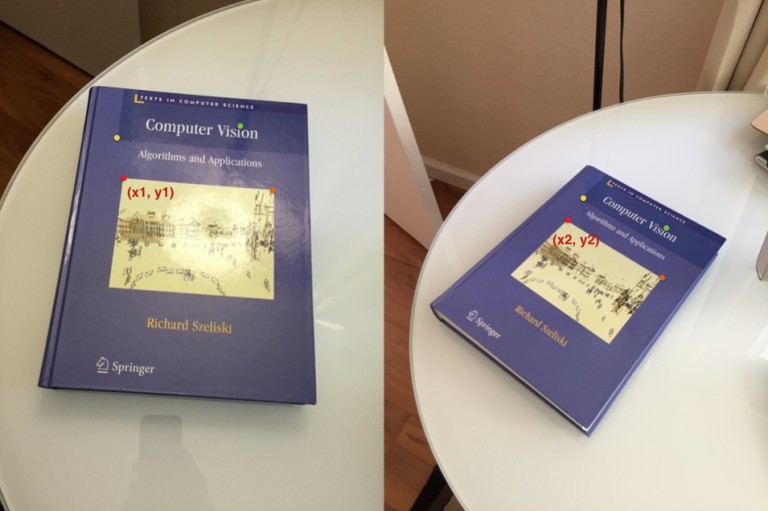
\includegraphics[width=15cm]{MasterThesis-master/images/homography_example.jpg}
    \caption{Point (x1,y1) on the book on the left image is corresponded to point (x2, y2) in right one.}
    \label{fig:homography_example}
\end{figure}

The formulation of homograph\ref{fig:homography_example} is $x' = \begin{bmatrix} A & t \\ 0 & 1 \end{bmatrix} x, x'= \begin{bmatrix} x1 & y1 & w' \end{bmatrix}^{T}, x= \begin{bmatrix} x2 & y2 & w \end{bmatrix}^{T}$.
As Fig.\ref{fig:homography_example} shows the homography matrix is the key to match correspondent points in both pictures.
Usually traditional algorithm try to find out the matrix by using SVD\cite{essig2010fully}.

\subsection{Random Sample Consensu}\label{section:RANSAC}
RANSAC is the short form of Random Sample Consensu\cite{wiki:RANSAC}.
This method is used to find the best model to fit data with noise.
In the dataset we have, we can connect the same object in different images.
As the result, many homograph matrices will be generated.
Among all the matrices generated, they should be seperated by or namly cleaned by some other algorithm.
RANSAC is the common algorithm to use to find out suitable homograph matrix.
It mainly discard the noise points in the data.
It is iterable, which means it can find out pattern between images and output the most suitable H homograph matrix.
Fig.\ref{fig:RANSAC} shows an example for RANSAC to find the linear pattern in all the data.

\begin{figure}[h!]
    \centering
    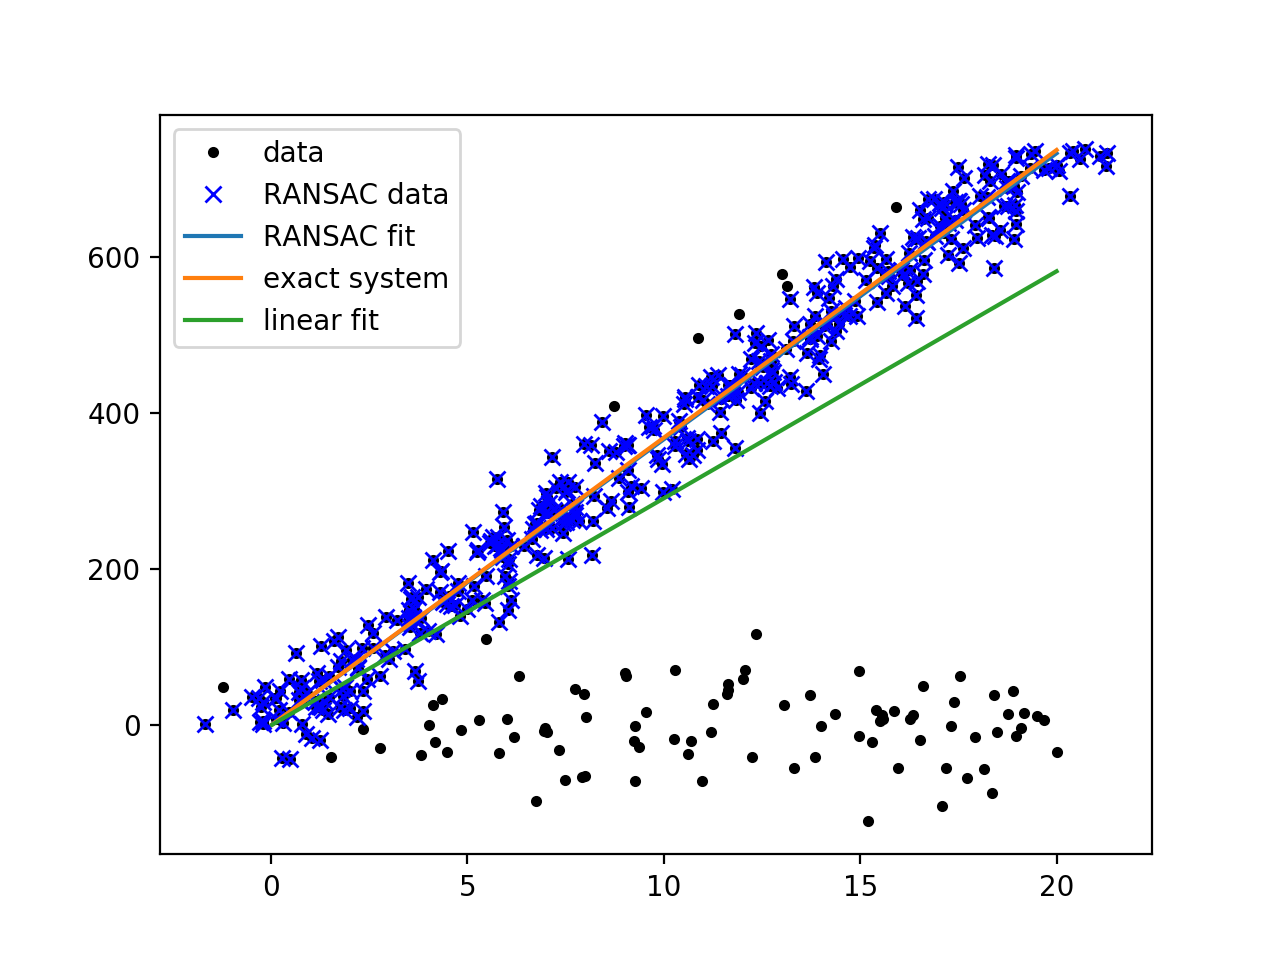
\includegraphics[width=15cm]{MasterThesis-master/images/RANSAC.png}
    \caption{Black points and blue cross points are the raw data, RANSAC tried to recognize noise in the data, and fit the rest correct data set with linear function line in green, and the ground truth line is showed in red.}
    \label{fig:RANSAC}
\end{figure}


\subsection{Camera Calibration}
Camera calibration is also called as pinhole camera model.
\begin{figure}[H]
    \centering
    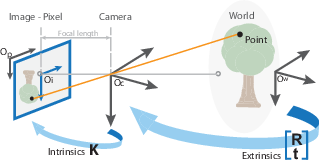
\includegraphics{MasterThesis-master/images/calibration_cameramodel_coords.png}
    \caption{Pinhole model from real world to images taken in camera.}
    \label{fig:pinhole_model}
\end{figure}
For most applications, pinhole camera model\ref{fig:pinhole_model} is accurate enough to mimic camera construction coordinate.
Usually, the relationship between points in real world and points in images can be described as formulation.$\lambda x = PX$ Fig.\ref{fig:pinhole_model_coordinate}.

\begin{figure}[h!]
    \centering
    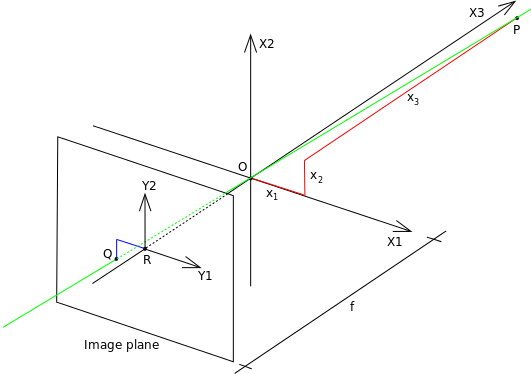
\includegraphics[width=10cm]{MasterThesis-master/images/Pinhole.png}
    \caption{Pinhole model.}
    \label{fig:pinhole_model_coordinate}
\end{figure}

X is the point in the real world, which is a 4 dimensional vector as $X = \begin{bmatrix} X & Y & Z & w \end{bmatrix}$.
x is the point in image, which is a point in the image, could be written as $x = \begin{bmatrix} x & y & w \end{bmatrix}$.
P is the camera calibration matrix, 
\begin{equation}\label{eq:1}
    P=K[R|t].
\end{equation}
In equation \ref{eq:1}, R is the rotation matrix to describe how much angle the object should rotate in the image.
t is the translation matrix shows the distance moved in the camera center.

\begin{equation}\label{eq:K}
    K=\begin{bmatrix} \alpha f& s & c_x\\ 0 & f & c_y\\ 0 & 0 & 1 \end{bmatrix}
\end{equation}
In equation \ref{eq:K}, distance between image plane and camera center is f.
s is the tilting parameter, usually it is set to 0.
With equation \ref{eq:K}, points in the image can be rotate within the stable connection of the real world's object.

%%%%%%%%%%%%%%%%%%%%%%%%%%%%%%%%%%%%%%%%%%%%%%%%%%%%%%%%%%%%%%%%%%%%%%%%%%%%%%%

\section{Application Scenes}
The eye gaze can be implemented in a lot of platforms.

\subsection{Computer Communication}
Using gaze as the fast object selection method to replace the mouse.\cite{Sibert:2000:EEG:332040.332445}
An application called MAGIC is used as the controller to trace pupil.\cite{Zhai:1999:MGI:302979.303053}
Both applications are developed by analyze the gaze data to figure out focusing point on the screen.
As shown in Fig.\ref{fig:eye_tracker}
\begin{figure}
    \centering
    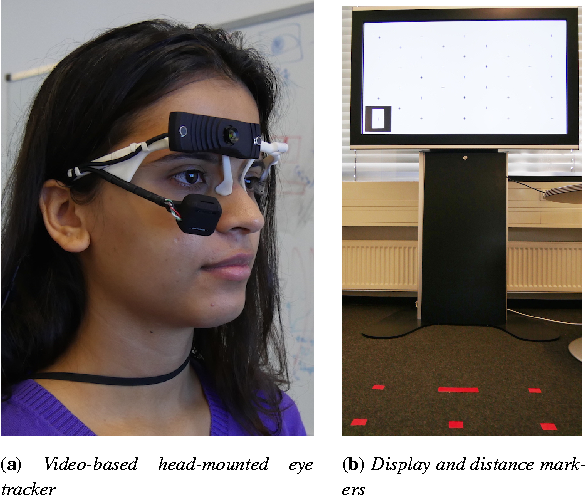
\includegraphics[width=9cm]{MasterThesis-master/images/eye_tracker.png}
    \caption{Video-based head mounted eye tracker}
    \label{fig:eye_tracker}
\end{figure}

\subsection{Display Panel Applications}
Long distance of eye gaze detection is also one important application.
As shown in Fig.\ref{fig:car_industry}
The techniques called corneal reflection is used to track gaze on large displays and smart TVs.
Combined with Adaboost and Shift algorithm, a robust pupil detection method is used to detect gaze.\cite{gwon2013robust}

\begin{figure}
    \centering
    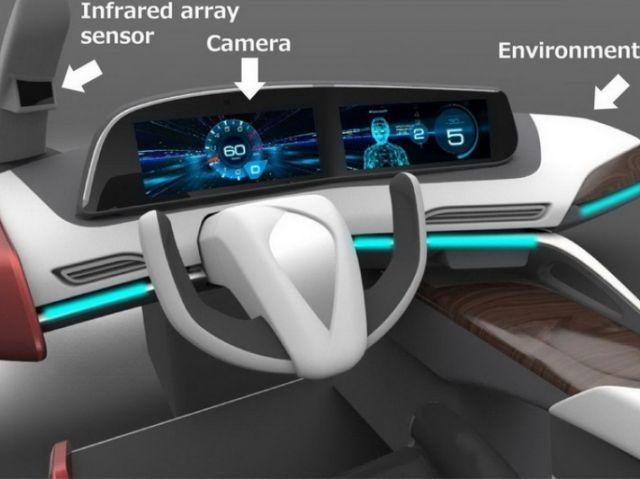
\includegraphics[width=9cm]{MasterThesis-master/images/car_industry.jpg}
    \caption{Car industry use to detect eye movement to keep driver safe.}
    \label{fig:car_industry}
\end{figure}

\subsection{Head-mounted setups}
With portable platforms devices, interactions can be used in VR, gaming controls, and AR.
As shown in Fig.\ref{fig:play_station}
Such 3D model mainly based on human head 3D models.
\begin{figure}
    \centering
    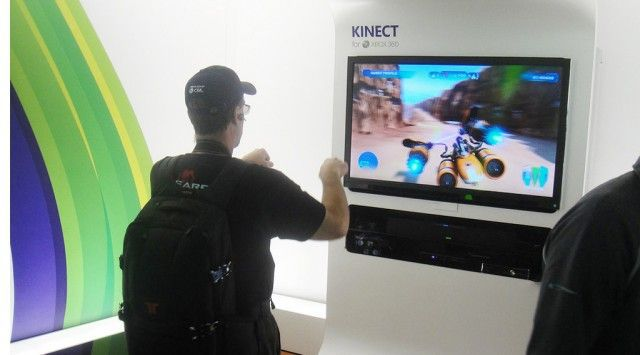
\includegraphics[scale=0.4]{MasterThesis-master/images/play_station.jpg}
    \caption{Play station use the gaze to make players more immersed in the enviorment.}
    \label{fig:play_station}
\end{figure}

%%%%%%%%%%%%%%%%%%%%%%%%%%%%%%%%%%%%%%%%%%%%%%%%%%%%%%%%%%%%%%%%%%%%%%%%%%%%%%%


\section{Organization of the thesis}
The rest of the thesis is structured as follow.
Chapter 2 will introduce related papers using convolution networks to detect gaze directions.
Include the papers shortages and advantages.
Besides that, the different structures in both traditional pipeline algorithm and end-to-end algorithms are explained in details.
In chapter 3 we describe our methodology used in the thesis.
From data collection to data cleaning.
And then the network structure we used in the thesis.
In chapter 4 we showed out the data structure and mainly detailed in training the network.
Finally, we compare our results with the others.

%%%%%%%%%%%%%%%%%%%%%%%%%%%%%%%%%%%%%%%%%%%%%%%%%%%%%%%%%%%%%%Chapter Related work
\chapter{Related Work} \label{related_work}
%%%%%%%%%%%%%%%%%%%%%%%%%%%%%%%%%%%%%%%%%%%%%%%%%%%%%%%%%%%%%%Chapter 3
The gaze estimation methods are mainly separated into two directions.
One is using pipeline structure as equation\ref{eq:1} and then equation \ref{eq:K}.
Equation \ref{eq:1} used to build transformation matrix between every images of the same person.
Equation \ref{eq:K} used to build transformation matrix between real world 3D points with images.
The steps can be described as below.
\begin{center}
    \smartdiagramset{back arrow disabled=true}
    \smartdiagram[flow diagram:horizontal]{Head Trackers, Equation \ref{eq:1}, Physical 3D Model, Equation\ref{eq:K}, Angles}
\end{center}

The second one is aiming to build one end-to-end algorithm.
Directly extract gaze direction from images.
Thus the process is different from pipeline model.
Based on training and learning processes.
Convolutional neural networks are good at looking for features by itself.
As the result, the neural networks end-to-end system can be described as below.
\begin{center}
    \smartdiagram[flow diagram:horizontal]{Images, CNN Network, output angles}
\end{center}

The training process is a circle.
Every image put inside the system will generate a label.
The label here is the angle of gaze direction.
Compare the label with the ground truth to optimize networks' weights.
After long time running we can get a suitable network.
%%%%%%%%%%%%%%%%%%%%%%%%%%%%%%%%%%%%%%%%%%%%%%%%%%%%%%%%%%%%%%%%%%%%%%%%%%%%%%%

\section{Traditional gaze estimation}
Because the lack of computer power, the traditional way is more focus on the mechanism of different filters.
In computer vision area, we choose features by designing a fixed weights filter.
The filter is some sort of matrix.
We use physical model to to setup specific relationship between images and real world object.
The pipeline system we built is not robust enough due to the complexity problems.
We have constraints on light, camera distance, human skin color and head rotation angle range.

Generally, we should first decide the eye movements types by calculating movement rates and duration of the movement.
The movements are shown in table \ref{tab:eye_movements}
\begin{table}[htbp]
    \centering
    \begin{tabular}{|l|l|l|l|l|}
        \hline
         Eye Movement & Movement rate & Duration  & Application \\\hline
         Fixation & < 15-100 deg/ms & 180-275 ms  & Browsing information\\\hline
         Saccade & 100-700 deg/sec & 20-200 ms &  Visual Search\\ \hline
         Smooth pursuit & <100 deg/sec & 100 ms &  Gazed based steering \\ \hline
         Scan path & -- & -- & Assessing user behavior \\ \hline
         Gaze duration& -- & -- &  Item Selection \\ \hline
         Blink & 12-15 per min & 300 ms &  Eye liveliness detection \\ \hline
         Pupil size change & 4-7 mm/sec & 140 ms & Assessing cognitive\\ \hline
    \end{tabular}
    \caption{Classification of Eye Movements}
    \label{tab:eye_movements}
\end{table}
Different types of movements can be coded into different models.
Using the model pipeline to fine tune until arrive the acceptable accuracy.


\subsection{Traditional Pipeline Algorithm}
\begin{center}\label{pipeline}
    \smartdiagramset{back arrow disabled=true}
    \smartdiagram[flow diagram:horizontal]{Position user in front of eye tracker, Estimate head pose in angles, Do user's ye calibration, Run head-based characterization, Save eye-tracking data, calculate gaze direction}
\end{center}
The pipeline algorithm is shown in \ref{pipeline}.
The first step needs devices eye tracker and camera.
The tracker will generate camera calibration matrix.
And the camera will record a video.
After that, use the head pose estimation model to get head pose angles.

\begin{table}[h]
    \centering
    \begin{tabular}{c|c|c}
         User parameters & Device parameters & Environment parameters \\ \hline
         Head pose & Number of cameras & Platform movement \\ 
         Eye occlusion & Camera resolution & Illumination changes \\
         Eye limitations & -- & Screen display size and resolution \\
         Hand pose/vibration & -- & User distance from tracker \\ 
    \end{tabular}
    \caption{Parameters of evaluate eye tracking systems}
    \label{tab:parameters}
\end{table}

The parameters in the table\ref{tab:parameters} are all needed for traditional algorithm.
Because of the large amount of parameters, the whole system is unstable.
The algorithm is specific to specific person.
Once you change the light or move yourself too much, the algorithm will likely to fail down.

\section{Deep learning based methods}
Deep learning has become more and more popular during these days.
Since 2012, the deep neural networks architectures have been popular since 2012.
The first neural network champion of Large Scale Visual Recognition Challenge(ILSVRC)\cite{ILSVRC15} is Alex Net.
It improved the result, from error rate 25.8 to error rate 16.4.
After 2012 the released of Alex net, the competition has been totally charged by convolution neural network structures as shown in Fig.\ref{fig:imagenet}.

\begin{figure}
    \centering
    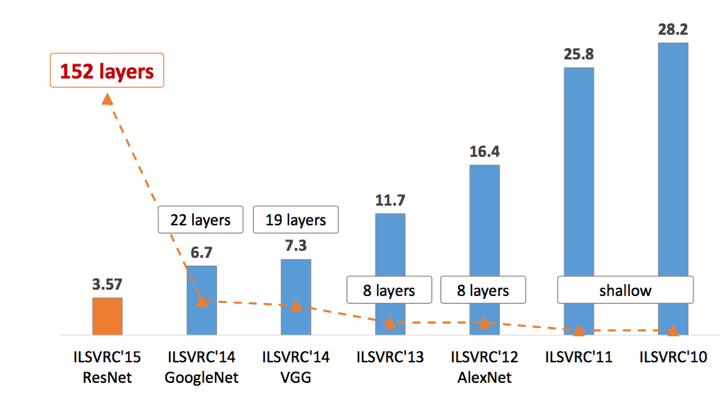
\includegraphics[width=15cm]{MasterThesis-master/images/cnnnetworks.png}
    \caption{Since the released of Alex net in 2012, image recognition area has turn to CNN structures.}
    \label{fig:imagenet}
\end{figure}

\subsection{Gaze Estimation in the Wild}
Paper \cite{zhang2015appearance} is the state of art method in 2015 in gaze estimation area.
It replaced some of the traditional pipeline into CNN structures.
The pipeline model is shown in Fig. \ref{fig:csm_pipeline}.
\begin{figure}[h]
    \centering
    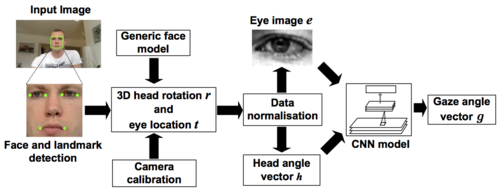
\includegraphics[scale=1.3]{MasterThesis-master/images/csm_MPIIGaze_pipeline.png}
    \caption{Pipeline model of MPIIGaze}
    \label{fig:csm_pipeline}
\end{figure}
The pipeline needs input images and then detected by using facial landmarks algorithms in paper \cite{li2013learning}.
As the first step, landmarks are the one kind of the inputs.
And then using generic face model and camera calibration together together to apply to the physical model.
After that, mixing camera calibration and face model together.
The coordinate and the face model is defined in paper \cite{Sugano2014LearningbySynthesisFA}.
Normalization is using the method proposed in paper \cite{Sugano2014LearningbySynthesisFA}.
It is aimed at using camera to look at the middle of the eye in a fixed distance, thus camera coordinate and head coordinate can be parallel.
The final step is calculating gaze angle vector from normalized data.
CNN model is shown in Fig. \ref{fig:cnn_model}
\begin{figure}[h]
    \centering
    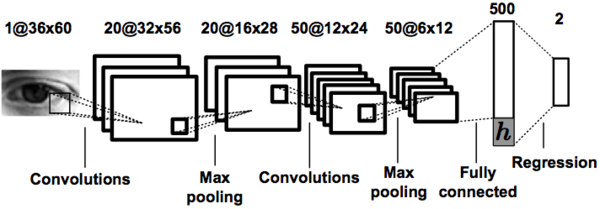
\includegraphics{MasterThesis-master/images/csm_MPIIGaze_cnnModel.png}
    \caption{The normalized eye image and head angle h are the inputs, through multi-cnn structure, the network will generate a angle vector.}
    \label{fig:cnn_model}
\end{figure}

The author had compared the network accuracy with the other pipelines algorithm in Fig.\ref{fig:compare}
\begin{figure}
    \centering
    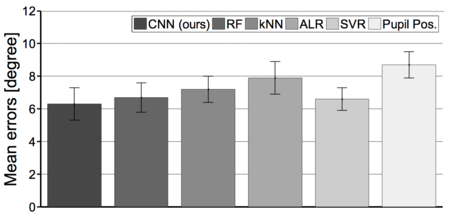
\includegraphics[scale=1.4]{MasterThesis-master/images/csm_MPIIGaze_within_MPII_dataset.png}
    \caption{Compare CNN part with different algorithms, the CNN model get the lowest error rate of 6.3.}
    \label{fig:compare}
\end{figure}
The CNN is a substitute of transitional RANSAC in section\ref{section:RANSAC}.
Multi-CNN model shows the power of solving complicated computer vision problems.
But this paper still using CNN as a part of the pipeline.
The input is still under a lot of constraints, which in the ideal situation should be limited to image only.

\subsection{Eye Tracking for Everyone}
In the paper <Eye Tracking for Everyone>\cite{krafka2016eye}, the structure is more useful to build an end-to-end algorithm.
The main idea of the paper is to eliminate camera calibration process and homograph process.
But the output of the algorithm is a different from paper \cite{zhang2015appearance}.
\begin{figure}[b]
    \centering
    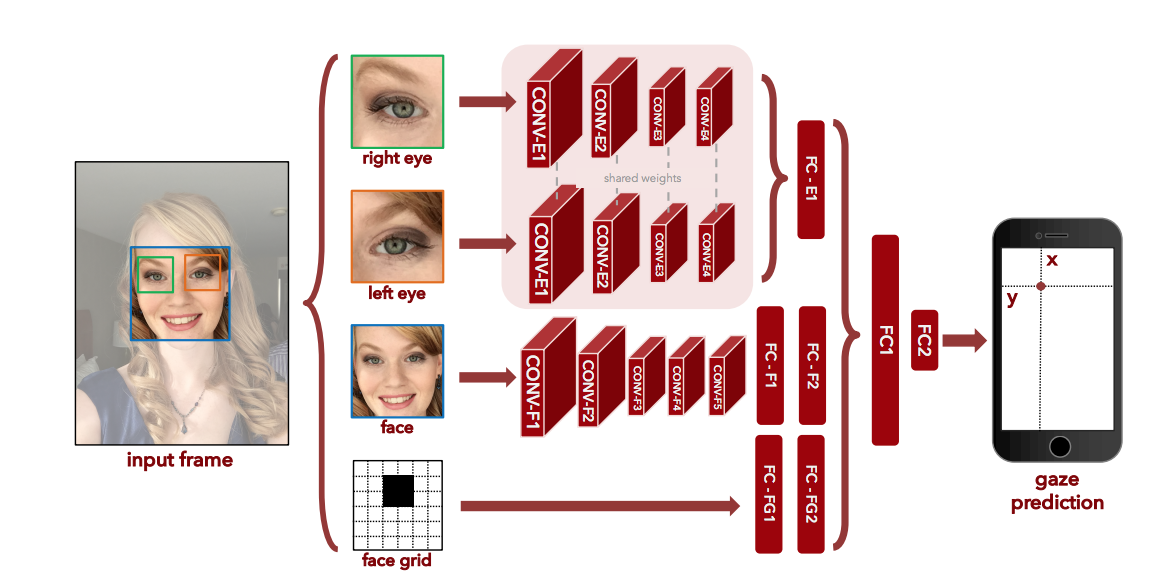
\includegraphics[width=15cm]{MasterThesis-master/images/eye_tracking_cnn.png}
    \caption{The CNN structure used in paper <Eye tracking for everyone> \cite{krafka2016eye}.The input is one image but divided in different four fields. The face grid in the image is used to emphasize face position in the image.}
    \label{fig:eye_tracking_CNN}
\end{figure}
As shown in the Fig.\ref{fig:eye_tracking_CNN}, the input image should be cut into 3 different parts.
The first two parts are right eye image and left eye images.
These kind of settings can enlarge the eye's resolution as the input of the network.
The face grid is one matrix of $25 \times 25$ pixels.
It is used to emphasize face location on the input frame.
Combine these four inputs together, the algorithm can generate points location on the screen.
The short coming of the algorithm is obvious too.
While training, you should use one specific person's data as input.
And also, the eyes' and face images should be cut off from face landmark detection algorithm.
Here they use dark net network \cite{hinton2015distilling} in their network in order to detect eyes.
The face is also detected by dark net network\cite{hinton2015distilling}.


\subsection{Compared existing methods}
So far for now, there are lots of algorithms aiming to deal with gaze recognition problems.
Basically it can be divided into different categories based on their setup equipment and usages.
The accuracy and tested condition are shown in table.\ref{tab:gaze_estimation_alforithms_categories}.

\begin{table}[h]
\centering
\resizebox{\textwidth}{!}{%
\begin{tabular}{@{}|l|l|l|l|@{}}
\toprule
Method category & Setup & Accuracy & Tested condition \\ \midrule
2D regression & Single camera, multiple LEDs with 2 face camera & 0.8 degree\cite{brolly2004implicit} & Limited head movements \\ \midrule
3D model & 4 cameras 2 LEDs, mirros & 0.6 degree \cite{beymer2003eye}& Head pose compensated \\ \midrule
Appearance based & 1 camera, NIR illuminator & 0.5 deg \cite{tan2002appearance}&  \\ \midrule
 & webcam & Recognition rate 97\% \cite{wu2014gaze} &  \\ \midrule
 & image database & Recognition rate 97\% \cite{george2016real}&  \\ \midrule
Cross Ratio based & 4 IR LEDs, 1 camera & 0.3-0.4 deg without headmovement \cite{huang2014towards}& Head movement allowed \\ \midrule
Shape based methods & 1 camera & 85\% \cite{wang2011driver}& None \\ \midrule
 & image frames & 4.5 pixels \cite{reinders1997eye}& None \\ \bottomrule
\end{tabular}%
}
\caption{Gaze estimation algorithms categories}
\label{tab:gaze_estimation_alforithms_categories}
\end{table}  
As the categories in  table\ref{tab:gaze_estimation_alforithms_categories}, it is easily to find that all the algorithm are testing in their own standard.
The reason is that the equipment are so different from each algorithms and the circumstances are also different.
Since all the details are different, we do not have a suitable testing cases for every algorithm.
It is actually a problem in gaze estimation area.

The main focus of our research is the appearance based eye gaze estimation algorithms\cite{zhang2015appearance}\cite{Sugano2014LearningbySynthesisFA}.
These algorithm are also variant.
Usually they should collect their own data set, like \cite{zhang2015appearance}, they collected data from web-cam of 15 persons using laptop.
In paper \cite{krafka2016eye} they collect data from 1474 people, and totally get 2,445,504 images in their dataset.
Besides the dataset, the input of these algorithms are different.
And even the purpose, the purpose are mainly divided into two parts.
One is the direction in three coordinate\cite{zhang2015appearance}, another is to predict the point on the screen\cite{krafka2016eye}.

%%%%%%%%%%%%%%%%%%%%%%%%%%%%%%%%%%%%%%%%%%%%%%%%%%%%%%%%%%%%%%%%%%%%%%%%%%%%%%%
\chapter{Methodology} \label{methodology}
%%%%%%%%%%%%%%%%%%%%%%%%%%%%%%%%%%%%%%%%%%%%%%%%%%%%%%%%%%%%%%%%%%%%%%%%%%%%%%%
\section{Network Structure} \label{network structure}
Our network is composed of three main part.
The first part is the pre-trained model.
And the second one is the attention mechanism model.
The last part is for regression of gaze direction.
The structure is simple and elegant.

Our main idea is follow the instinct of human gaze seeing process.
First, using feature extract structure to recognize features on the face.
The features trained by the other recognition algorithms can be transferred to our network by using transfer learning technique described in Chapter \ref{cha: transfer learning}.
So that the first part of the network can recognize the face landmarks like eyes.
Then, in order to focus on the some important region or what we may consider as the interest region.
We try to use attention mechanism as described in chapter \ref{cha: attention model}.
The mechanism is a 1x1 kernel convolution network, it is used to extract previous pre-trained model's output to generate a 13x13 feature map.
The feature map can be used to add weights to the original pre-trained output.
After feature extraction and weight enhancement, we use two fully connective layer to regress the gaze direction.

\begin{figure}[b]
    \centering
    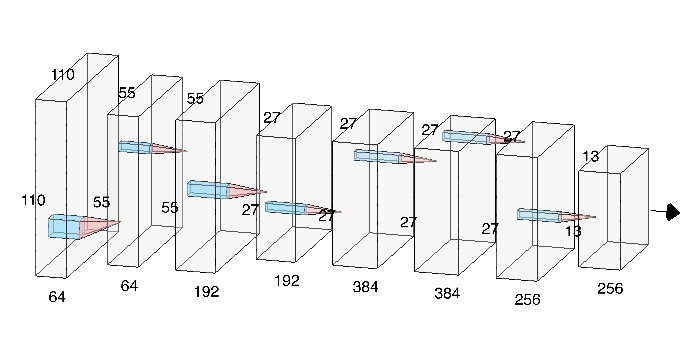
\includegraphics[width=15cm]{MasterThesis-master/images/pre_trained.jpg}
    \caption{Pre-trained model, similar to Alex net.}
    \label{fig:pre_trained_model}
\end{figure}

\subsection{Transfer Learning}\label{cha: transfer learning}
The lower layers in CNN algorithm structure are doing the similar things.
To be more detailed as describe in \cite{noh2015learning}.
It explains the common features of CNN, which the lower layers are extracting simple features like line, circle or rectangles.
And due to this trait of CNN, it is possible to transfer a trained network to the other networks.
The lower part of the CNN model is able to distinguish different objects even if your target objects are not included in their labels. 
\begin{figure}
    \centering
    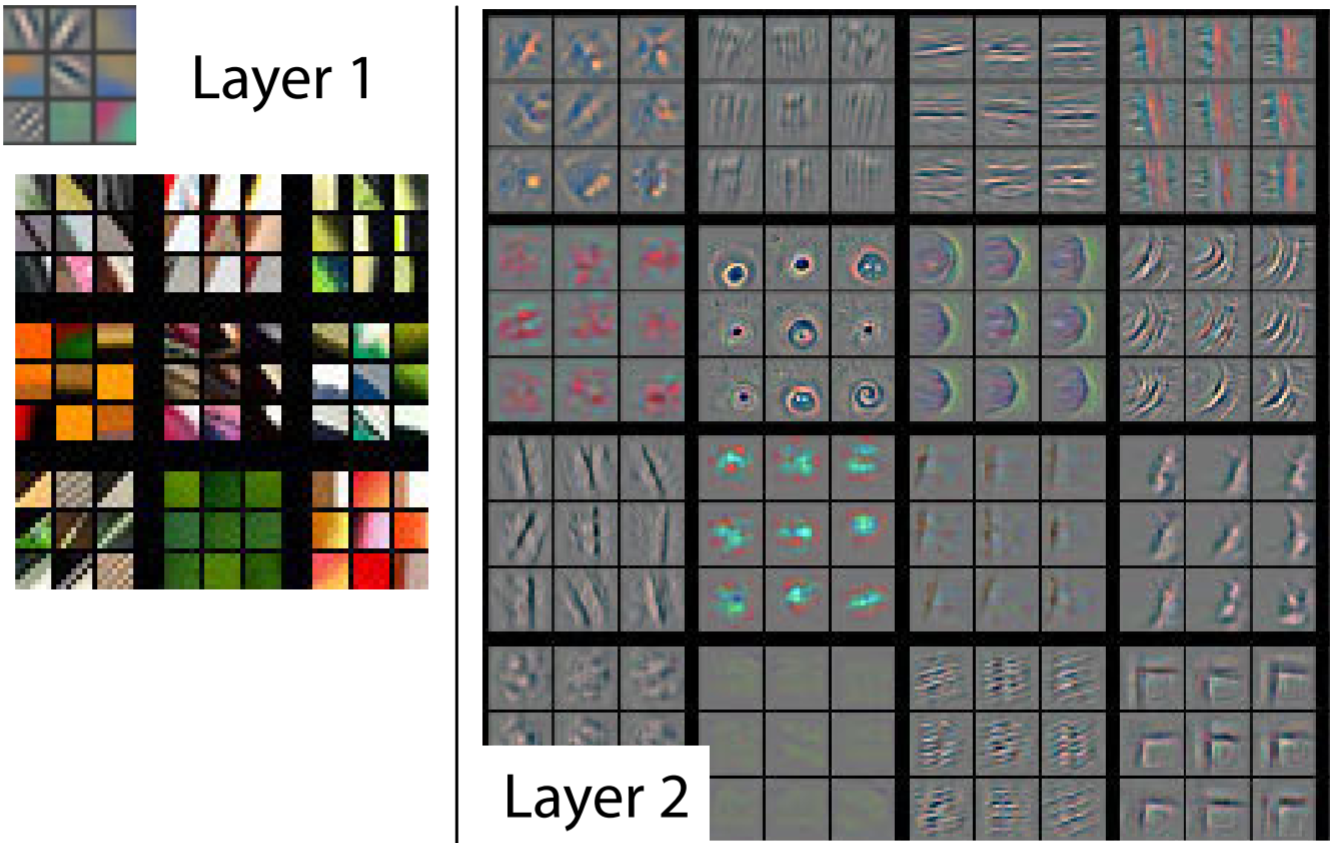
\includegraphics[width=15cm]{MasterThesis-master/images/deconv.png}
    \caption{DeConvNet illustrates features extracted by CNN.}
    \label{fig:deconv}
\end{figure}

As showing in Fig.\ref{fig:deconv}, the first layer is detecting simple pattern in images.
And then when the layer becomes more deeper, the features become more complex.
As the result, we can use the first few layers to extract features.
Because basic features like lines or basic shapes are the same.


\subsection{Pre-trained Model}
Here is the pre-tranined model Fig.\ref{fig:pre_trained_model}.
It is similar to Alexnet\cite{krizhevsky2012imagenet}, the Alex net model get a very high precision, error rate of 0.16422, in 2012  ImageNet Large Scale Visual Recognition Competition.
Compared to the other competition winners, it occupies less space which means higher processing speed.
In the pre-trained model Fig.\ref{fig:pre_trained_model}, the input image size is 448x448x3.
After convolutional neural network it will output a 13x13x256 feature map, which means a 13 width and 13 height 256 depth wrights.
As in the original paper, this algorithm is aiming to classify 10,000,000 labeled images depicting 10,000+ object categories\cite{ILSVRC15}.

\subsection{Attention Model}\label{cha: attention model}
\begin{figure}[h]
    \centering
    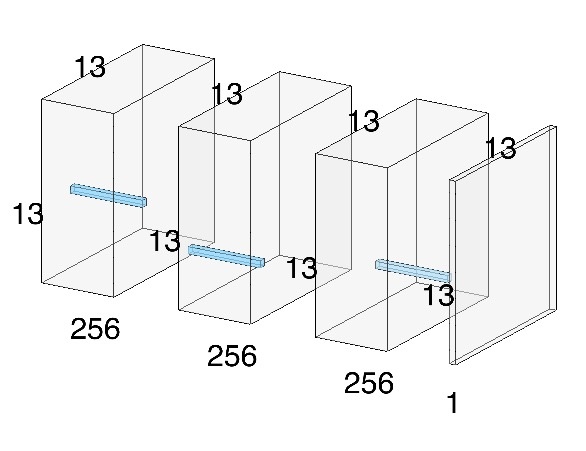
\includegraphics[width=10cm]{MasterThesis-master/images/attension.jpg}
    \caption{Attention model}
    \label{fig:attention model}
\end{figure}

The output as from pre-trained model (Fig.\ref{fig:pre_trained_model}) is a feature map matrix U with shape of 13x13x256.
The attention model's output is a matrix W with shape of 13x13x1.
Using element wise multiplication equation \ref{eq: attention model}, output matrix V has the same shape of W.
\begin{equation}\label{eq: attention model}
U \odot W = V
\end{equation}

The attention model used conv 1x1 kernel with stride 1.
And then use Relu as equation \ref{eq: attention model} to activate each layer's output.
\begin{equation}\label{eq:relu}
    f(x)= 
\begin{cases}
    x,& \text{if } x\geq 0\\
    0,              & \text{otherwise}
\end{cases}
\end{equation}

\subsection{Fully Connected Layer}\label{cha: fcn}
After extracting features from pre-trained model (chapter \ref{cha: transfer learning}), use the output of the extracted feature as the input to attention model in chapter \ref{cha: attention model}.
Calculate the matrix V (equation \ref{eq: attention model}), the V matrix is the preferred feature to represent the eye gaze.
Thus, the last step is to do regression operation.
This step is mainly to generate a appropriate label.
We use two fully connected layers to do the regression work.
\begin{figure}
    \centering
    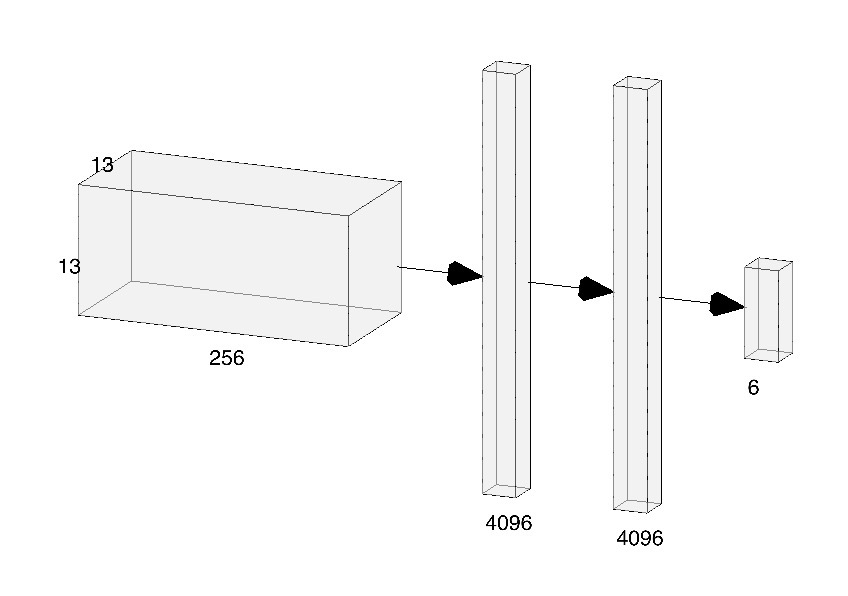
\includegraphics[width=10cm]{MasterThesis-master/images/fcn.jpg}
    \caption{Fully Connected Layers}
    \label{fig:fcn}
\end{figure}
In order to get the appropriate shape, we transformed the V matrix from shape 13x13x256 to 43264x1.
And then the reshaped matrix can be connected to fully connected layers and generate a 6 dimensional matrix represent points on the screen.

\section{Training Phase}
\subsection{Data Augment}
We use a set of data augments methods to deal with different illumination.
In order to re-size input image to the same size of 448x448, we use bi-linear interpolation.
Because bi-linear interpolation algorithm is continuous, the visual effect is better than the other re-size algorithm like KNN\cite{han2013comparison}.
And also the bi-linear interpolation is faster than bi-cubic interpolation algorithm.
Therefore the bi-linear algorithm is a speed and clarity compromise.

Another problem we should consider is the illumination.
Focus on illumination we come up with two specific solution.
One is brightness, and the other one is color.
We use random brightness chosen method based on the equation \ref{brightness}.
\begin{equation}\label{brightness}
    j(x, y) = \alpha f(x, y) + \beta
\end{equation}
The $\alpha, \alpha \geq 0$ here represents the contrast of one image.
We use the constant value.
And $\beta$ is a randomly chosen value from -0.5 to 0.5.
In equation \ref{brightness}, the f(x,y) represents one pixel value in the original input image.
j(x,y) represent the output of a altered image pixel.

For the color space, first we change the RGB color space to HSV by equation \ref{eq:hue}, and then randomly add a value to Hue axis.
R, G, B are the three channels values in each pixel, $h_{RGB}$ is the converted hue value.

With combing these two methods together, we can largely change the brightness and color of the original images. 
\begin{equation}\label{eq:hue}
    tan(h_{RGB}) = \frac{\sqrt{3}(G-B)}{2R-G-B}
\end{equation}

\subsection{Loss Function}
Considering our output value, we try to use Mean Square Error as our loss function.
For each image input x, our output $\hat{\theta}_m$ is a 6 dimension vector $\hat{\theta}_m\in R^{1\times 6}$.
The ground truth is the same dimension vector $\theta$.
The loss function can be written as equation \ref{eq:loss function}.
\begin{equation}\label{eq:loss function}
    MSE=\frac{1}{n}\sum_{i=1}^n (\hat{\theta}_i - \theta)^2
\end{equation}
% Besides MSE, absolute value can also be written in the paper.
The training phase will calculate derivation of loss function.

\section{Testing Phase} \label{testing phase}
During the test phase, we have two different kinds of tests.
One is for single person output.
And the other one is for multiple person output.
In the testing phase, we only need to input images and use forward inference procedure.
The image calculated through pre-trained model and then the 
The reason why we choose two different testing phase is mostly based on the skewing data we get.
The dataset details will be explained in section\ref{sec: dataset}.


%%%%%%%%%%%%%%%%%%%%%%%%%%%%%%%%%%%%%%%%%%%%%%%%%%%%%%%%%%%%%%%%%%%%%%%%%%%%%%%
\chapter{Experiments} \label{experiments}
\section{Images in MPIIGaze}\label{sec: dataset}
The dataset MPIIGaze contained 213,659 images collected from 15 laptop users over several months.
It covers a realistic reliable variability in appearance and illumination and therefore represents a significant big amount of data.
\begin{figure}
    \centering
    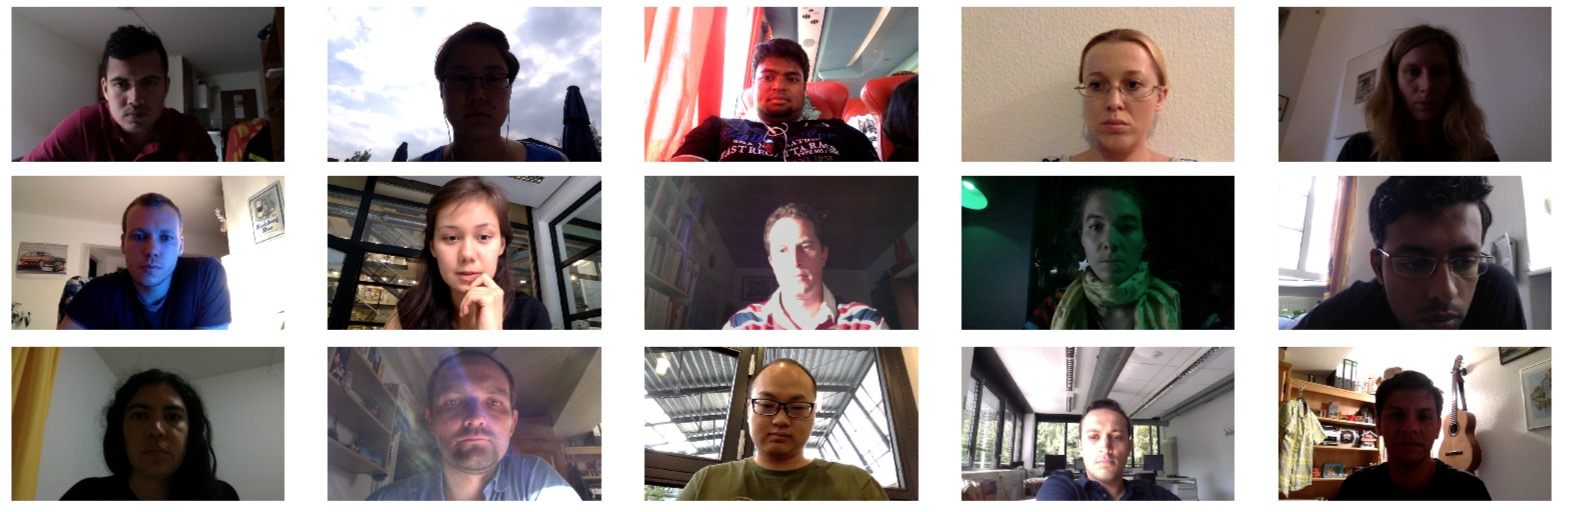
\includegraphics[width=15cm]{MasterThesis-master/images/head_images.jpg}
    \caption{Sample images from MPIIGaze dataset showing the considerable variability in terms of place and time of recording , directional light and shadows.}
    \label{fig:head images}
\end{figure}
The variety of the dataset can cover a vast range of illumination and usage situations.
Thus the dataset provide enough data to get algorithm trained on it.

\section{Dataset Structure}
For every image input, the dataset has 25 dimensions as shown in table\ref{table: annotations}.

\begin{table}[h]
\centering
\begin{tabular}{|l|l|}
\hline
Dimension  & Explaination                                                     \\ \hline
1          & Image file from path and name.                               \\ \hline
2$\sim$3   & Gaze location on the screen coordinate in pixels.           \\ \hline
4$\sim$15  & (x, y) position for the six facial landmarks.                \\ \hline
16$\sim$21 & The estimated 3D head pose in the camera coordinate system. \\ \hline
22$\sim$24 & Face center in the camera coordinate system.                  \\ \hline
25         & Which eye is used for the evaluation subset.                \\ \hline
\end{tabular}
\caption{MPIIGaze Annotations}
\label{table: annotations}
\end{table}

\section{Pre-trained model VGG VS AlexNet}
% Calculate number of wrights 
% Scale up eye region.
VGG is also one famous image classification structure\cite{simonyan2014very}.
\begin{figure}[h]
    \centering
    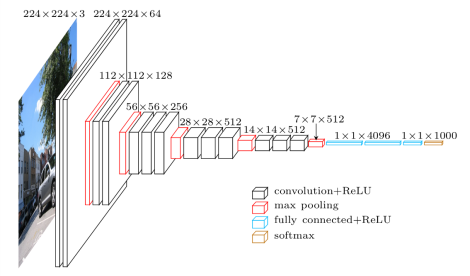
\includegraphics[width=10cm]{MasterThesis-master/images/vgg16.png}
    \caption{VGG16 Structure}
    \label{fig:VGG16}
\end{figure}
The structure of VGG net has more parameters and occupy a more larger space.
But for small objects like eyes, the VGG structure use the 3x3 conv operation.
Contrast with AlexNet, which used a 11x11 conv operation, VGG has a receptive field smaller than AlexNet.
A smaller receptive field means the more detailed regions can be detected.
As the pupil is in the middle of the eyes.
VGG can be more accurate in detecting the small pupil.
But the shortcoming is also obvious.
VGG has two times amount of weights than AlexNet, the testing speed is slower and need more computing power inside GPU.
VGG has 138 million parameters compared  AlexNet with million.
Thus we use these two pre-trained model and test it together to get results.

% Batch size

\section{Fine tuning model}
% dropout
% batch norm
% learning rate
Because our dataset contained 213,659 images of 15 persons, for every person, they have 14000 on average.
The image's input is a size of 448x448.
Because of the big amount of data, we need to avoid overfit at the beginning.
Refering to the paper Hinton et.al 2012\cite{DBLP:journals/corr/abs-1207-0580}, we use dropout layer in the fully connected layers.
The basic idea of dropout layer is that, during training phase, randomly dropout some nodes in the network based on equation.
\begin{equation}\label{eq: dropout}
\begin{array}{l}
     r_{j}^{(l)} \sim Bernoulli(p)\\
    \Tilde{y}^{(l)} = r^{(l)} \times y^{(l)} \\
     z_i^{(l+1)} = w_i^{(l+1)}\Tilde{y}^(l) + b_i^{(l+1)}\\
     y_i^{(l+1)} = f(z_i^{(l+1)})
\end{array}
\end{equation}
The model of dropout will randomly choose 1 or 0 from Bernoulli distribution.
After choose the value of one front layer and then multiply the 0, the node's output will be 0.
We add dropout layer in the fully connected layer to avoid overfit during training.
And for the large size of input image, we choose to use batch size of 8.
The memory is not allowed for a more larger network to work.
As for the learning rate, we use learning rate decay algorithm Adam\cite{kingma2014adam}.
\begin{figure}
    \centering
    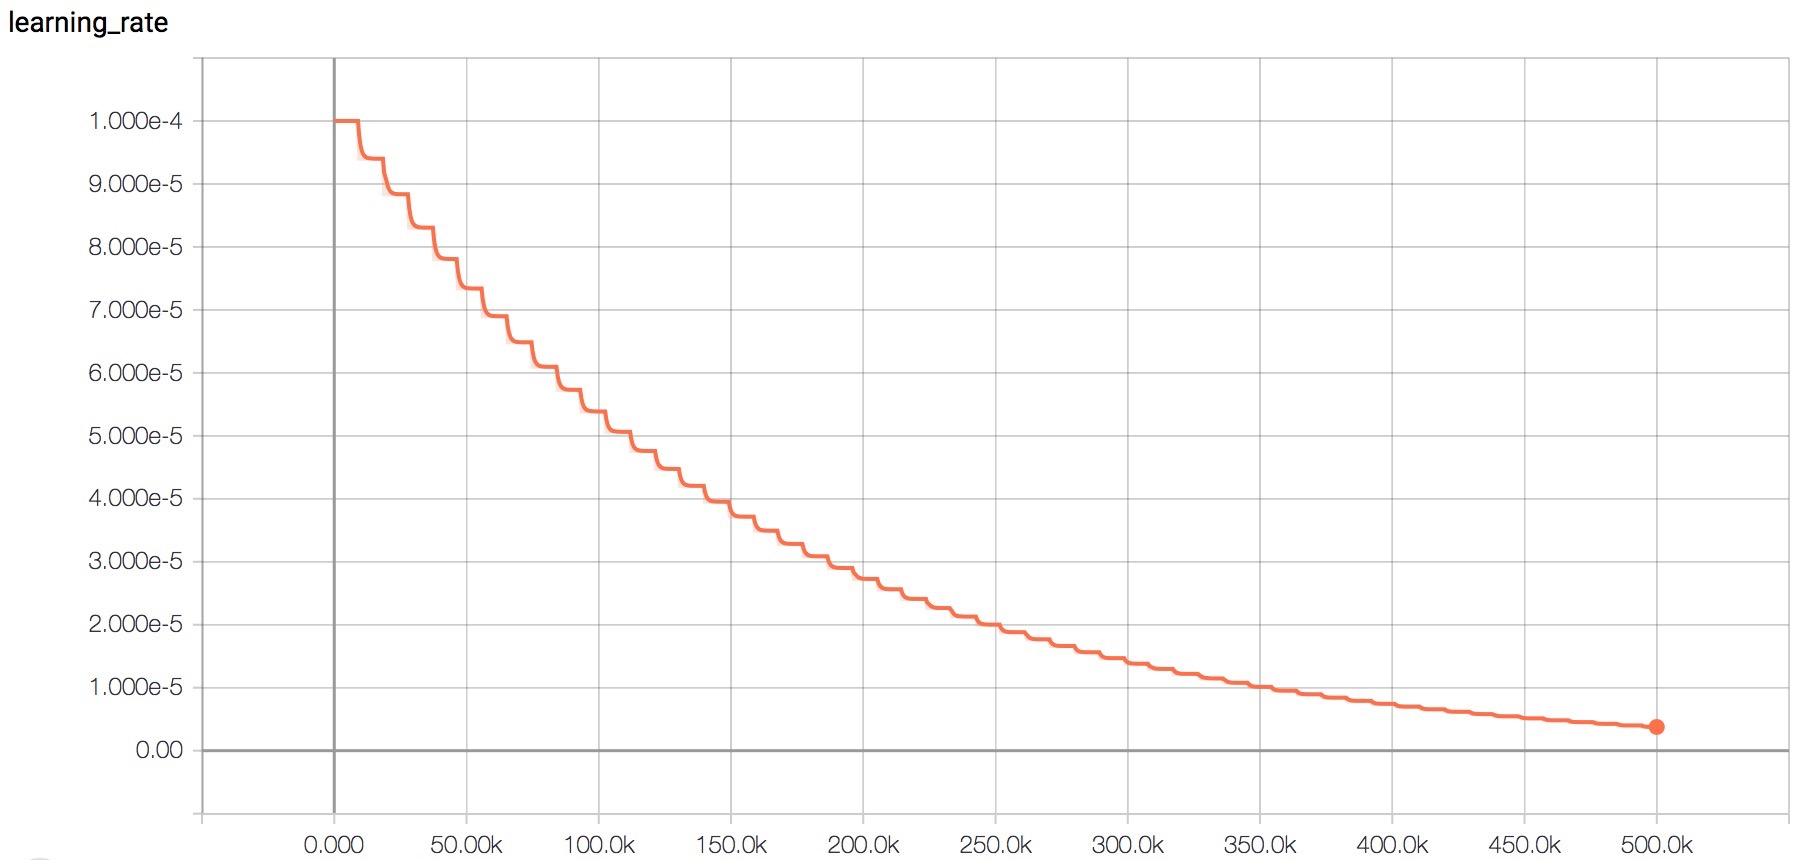
\includegraphics[width=15cm]{MasterThesis-master/images/learningrate.jpg}
    \caption{Learning rate in 500000 rounds changing curve VS steps.}
    \label{fig:learning rate}
\end{figure}
The Fig. \ref{fig:learning rate} shows the changing curve during 500000 steps.

% training time cost
Training the algorithm for 500000 rounds, we can decrease the loss to around 10.
It takes arounf 8 days to train, the loss changing log is shown in Fig. \ref{fig:loss}.
\begin{figure}
    \centering
    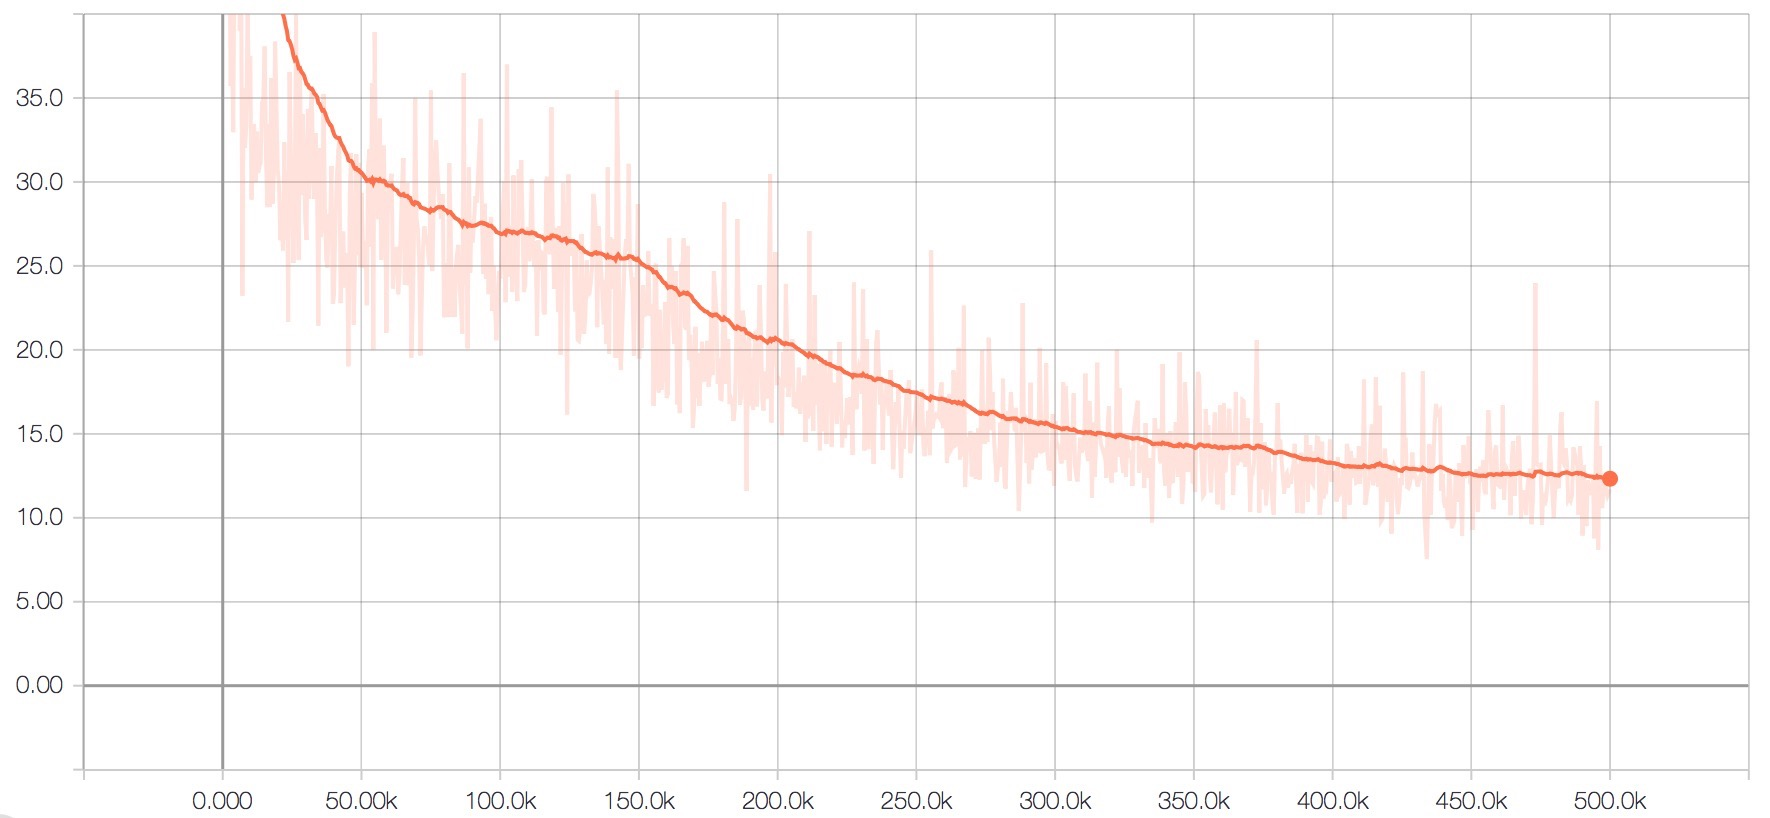
\includegraphics[width=15cm]{MasterThesis-master/images/loss.jpg}
    \caption{Total loss changing curve VS steps}
    \label{fig:loss}
\end{figure}

\section{Hyper Parameters}
%batch size 
% SGD
Batch size is one important parameter here, it is mainly depends on the memory of the GPU.
Here we use GPU 1080Ti with total memory 11172 MiB.

\section{Accuracy Metrix}
The accuracy is calculated by computing the degree difference between predicted vector and ground truth label.

\begin{equation}\label{accuracy}
\begin{split}
    cos\theta & = \frac{\hat{\theta}\theta}{|\hat{\theta_i}||\theta|} \\
        \theta      & = \begin{bmatrix} x_1 &x_2 &x_3 & x_4 &x_5 &x_6 \end{bmatrix}  \\
        \hat{\theta} & = \begin{bmatrix} {x_1}' &{x_2}' &{x_3}' & {x_4}' &{x_5}' &{x_6}' \end{bmatrix} 
\end{split}
\end{equation}

\section{Speed}
\section{Results Display}


\chapter{Future Work}\label{future work}
% Attention model Change relu to xsigmoid.
% model distill
% 
\bibliographystyle{IEEEtran}
\bibliography{LUOreference}
\end{document}
